%% ---------------------------------------------------------------------
%% ICIC 2026 submission, built on the conference's own ICIC2026.cls.
%%
%% The earlier version was built on plain IEEEtran and failed desk
%% screening: US Letter instead of A4, Computer Modern mathematics instead
%% of the Times-matched newtxmath the class loads, "Index Terms" instead of
%% "Keywords", a bold abstract, and no paragraph spacing. All of those come
%% from the class now, which is why the class must not be edited.
%%
%% TO BUILD ON OVERLEAF
%%   1. Upload ICIC2026.cls, this file, and a folder named  figures
%%      containing session_13-48_compact.png, doppler_by_acquisition.png
%%      and recovery_by_acquisition.png.
%%   2. Set this file as the main document. Compiler: pdfLaTeX.
%%
%% BLIND REVIEW. \blindtrue hides the author block and the repository URL.
%% The CMT portal states double-blind review while the template supplies
%% author blocks; confirm with the track chair which the desk-screening
%% copy should carry. \blindfalse below shows the authors.
%% ---------------------------------------------------------------------
\documentclass{ICIC2026}

%% The class supplies graphicx, amsmath, booktabs, cite and url. Only the
%% packages this manuscript adds on top of it are loaded here; nothing in
%% the class is overridden.
%% amssymb is not loaded: newtxmath already provides the AMS symbols and
%% the two clash over \Bbbk. Nothing in this manuscript needs it.
\usepackage{tikz}
\usetikzlibrary{arrows.meta,positioning}
\graphicspath{{figures/}}

%% The class numbers subsection HEADINGS A, B, C, as the template shows,
%% and \thesubsection therefore carries no section prefix. That is correct
%% for the heading but makes \ref{} print a bare "A", which is ambiguous
%% across five sections. \p@subsection prefixes the reference only, so the
%% headings still read "A." while a cross-reference reads "IV-A".
\makeatletter
\renewcommand\p@subsection{\thesection-}
\makeatother

\begin{document}

\title{Acquisition-Level Evaluation of Deep Learning for Range-Doppler Radar Target Recognition}

\newif\ifblind
\blindfalse

\ifblind
  \newcommand{\codeurl}{a repository archived with the submission}
  \author{}
\else
  \newcommand{\codeurl}{\url{github.com/falcon-colab/rdrd-acquisition-coverage}}
  \author{%
  \ICICAuthorRowThree
    {\ICICAuthorBlock{Ghulam Mustafa}{College of Aeronautical Engineering}{National University of Sciences and Technology}{Islamabad, Pakistan}{gmustafa.ms19avecae@student.nust.edu.pk}}
    {\ICICAuthorBlock{Ghulam Murtaza}{College of Aeronautical Engineering}{National University of Sciences and Technology}{Islamabad, Pakistan}{murtaza.sab2@gmail.com}}
    {\ICICAuthorBlock{Ali Nawaz}{College of Aeronautical Engineering}{National University of Sciences and Technology}{Islamabad, Pakistan}{alinawaz1302@gmail.com}}
  \ICICAuthorRowTwo
    {\ICICAuthorBlock{Salman Liaquat}{College of Aeronautical Engineering}{National University of Sciences and Technology}{Islamabad, Pakistan}{salmanliaquat@ieee.org}}
    {\ICICAuthorBlock{Raja Farrukh Ali}{College of Aeronautical Engineering}{National University of Sciences and Technology}{Islamabad, Pakistan}{rfali@cae.nust.edu.pk}}
  }
\fi

\maketitle

\begin{abstract}
Public radar target recognition benchmarks are usually evaluated by randomly splitting individual range-Doppler frames, even though these frames come from continuous recordings. Such frame-level accuracy can hide how a classifier behaves on recordings it has never seen. This paper audits the Real Doppler RAD-DAR database at the acquisition level. Duplicate files are removed, 52 acquisitions are recovered from the directory structure, and a compact convolutional network is evaluated with acquisition-grouped five-fold cross-validation, a training coverage test, and an approximate three-frame input. Grouped partitioning lowers aggregate accuracy only from 0.934 to 0.910, a change smaller than the variation between folds. The per-acquisition breakdown tells a different story. Twenty of the twenty-one drone acquisitions exceed 0.90 recall, whereas one reaches only 0.249. With this acquisition held out of training, recall on a reserved half is 0.178. Adding its other half to training raises recall on the same half to 0.948, and repeating the test for all 52 acquisitions produces no comparable case. The failing acquisition can be identified before training from the Doppler position and spread of its energy. A three-frame input raises random-split accuracy to 0.979 but leaves this acquisition at 0.367. Per-acquisition recall, which costs a single cross-validation pass, should therefore accompany aggregate accuracy for any benchmark built from continuous recordings.
\end{abstract}

\begin{IEEEkeywords}
Cross-validation, data leakage, drone classification, evaluation protocol, FMCW radar, micro-Doppler, radar target recognition
\end{IEEEkeywords}

% =====================================================================
\section{Introduction}

Radar surveillance of drones, vehicles, and pedestrians increasingly relies on deep networks trained on range-Doppler or micro-Doppler data~\cite{ahmad2024,liaquat2025imm,mustafa2026}. Published classifiers on the Real Doppler RAD-DAR database, a widely used frequency-modulated continuous-wave (FMCW) benchmark, report accuracies between 98\% and 99\%~\cite{roldan2020,zhang2025}. Such figures suggest that recognition on this sensor is nearly solved. This paper shows that the same level of accuracy can coexist with an almost complete failure on one recording, and that the usual evaluation protocol does not reveal it.

The cause lies in how the data are partitioned. Both published figures come from shuffling individual range-Doppler frames, although the dataset consists of continuous recordings whose consecutive frames are strongly correlated. Random partitioning therefore places frames of the same acquisition in both the training and test sets, so the reported accuracy measures performance on recordings the model has already seen. Grouped partitioning is the standard remedy~\cite{kapoor2023,buchman2022}, and this paper examines what it reveals. On this benchmark, grouped partitioning barely changes aggregate accuracy, which might suggest that the benchmark is sound. A per-acquisition breakdown shows otherwise. One drone acquisition has a recall of only 0.249, while every other drone acquisition exceeds 0.90. Aggregate accuracy does not merely understate this failure. It conceals it.

The contributions are fourfold. First, a reproducible preparation removes duplicates from the distributed archive and recovers the acquisition structure from its directory hierarchy (Section~\ref{sec:method}). Second, random and acquisition-grouped partitioning are compared over five folds and three seeds (Section~\ref{sec:leak}). Third, a controlled coverage experiment, repeated for all 52 acquisitions, shows that the failure stems from missing training coverage rather than intrinsic difficulty, and a descriptive signature identifies the acquisition without reference to classifier output (Sections~\ref{sec:distinguish}, \ref{sec:coverage} and~\ref{sec:controls}). Fourth, the failure is shown to persist with an approximate three-frame input that reaches 0.979 random-split accuracy (Section~\ref{sec:inputgap}). The audit procedure is independent of the dataset and applies to any benchmark built from continuous recordings.

% =====================================================================
\section{Literature Review}
\label{sec:related}

The Real Doppler RAD-DAR database was released with a convolutional baseline, DopplerNet, which reached 99.48\% accuracy in classifying vehicles, drones, and pedestrians~\cite{roldan2020}. The acquisition hardware is described separately~\cite{quevedo2019}. A recent lightweight model reached 98.08\% on the same data with a model size of about 400\,kB~\cite{zhang2025}. These studies belong to a broader line of work on convolutional networks for micro-Doppler signatures, which began with human activity classification~\cite{kim2016} and now covers drones~\cite{ahmad2024}, drones versus birds~\cite{mustafa2026}, and material classification with software-defined radio (SDR) platforms~\cite{liaquat2025imm}. End-to-end simulation of the range-Doppler and constant false alarm rate (CFAR) processing chain~\cite{liaquat2024tut} makes such datasets easier to produce, which raises the importance of how they are evaluated.

Correlated samples inflate performance metrics. Human activity recognition commonly uses subject-disjoint splits, and radar recognition studies use track-level separation for the same reason~\cite{buchman2022}. In WiFi sensing benchmarks, re-splitting by subject reduced reported performance to between roughly one quarter and three quarters of the published values~\cite{varga2024a,varga2024b}. A survey of leakage in machine-learning-based science provides a taxonomy~\cite{kapoor2023}. In that taxonomy, the duplicated archive tree described in Section~\ref{sec:method} falls under L1.4 (duplicates in the dataset), and random partitioning of correlated frames falls under L3.2 (nonindependence between training and test samples). Conditions absent from training have been addressed through single-source domain generalization for low-slow-small radar targets~\cite{chen2025} and open-set recognition, which rejects classes never seen in training~\cite{bai2026}. The present case is different. The failing acquisition is correctly labeled and its samples lie closest to the drone centroid, so it is a closed-set acquisition shift, in which a known class contains a scenario absent from the training split.

Comparing learning procedures across resampled partitions is statistically delicate. Common tests have inflated Type~I error on cross-validation scores~\cite{dietterich1998}, and variance estimates must account for overlapping training sets~\cite{nadeau2003}. In computer vision, compression has been found to affect some classes disproportionately~\cite{hooker2019,tran2022}. Section~\ref{sec:discussion} reports a related observation for radar at the level of individual acquisitions.

% =====================================================================
\section{Methodology}
\label{sec:method}

\begin{figure*}[t]
\centering
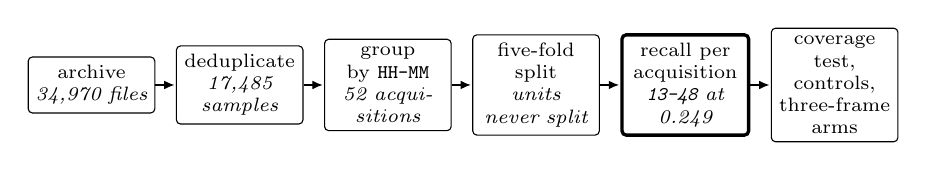
\begin{tikzpicture}[
  bx/.style={draw, rounded corners=1.5pt, align=center, inner xsep=2pt,
             inner ysep=3pt, text width=0.121\textwidth, font=\scriptsize},
  hl/.style={bx, very thick},
  ar/.style={-{Latex[length=1.3mm,width=1.1mm]}, shorten >=0.5pt}]
\node[bx] (a) {archive\\{\itshape 34,970 files}};
\node[bx, right=2.6mm of a] (b) {deduplicate\\{\itshape 17,485 samples}};
\node[bx, right=2.6mm of b] (c) {group by \texttt{HH-MM}\\{\itshape 52 acquisitions}};
\node[bx, right=2.6mm of c] (d) {five-fold split\\{\itshape units never split}};
\node[hl, right=2.6mm of d] (e) {recall per acquisition\\{\itshape \texttt{13-48} at 0.249}};
\node[bx, right=2.6mm of e] (f) {coverage test, controls,\\three-frame arms};
\draw[ar] (a) -- (b); \draw[ar] (b) -- (c); \draw[ar] (c) -- (d);
\draw[ar] (d) -- (e); \draw[ar] (e) -- (f);
\end{tikzpicture}
\caption{Preparation and evaluation pipeline. The bold step is not produced by a frame-level protocol and adds no training cost. Each unit is held out exactly once, so one cross-validation pass yields the recall of every acquisition and reveals \texttt{13-48}.}
\label{fig:pipeline}
\end{figure*}

Fig.~\ref{fig:pipeline} summarizes the preparation and evaluation pipeline described in this section.

\subsection{Dataset}

The database was collected with an FMCW radar operating at 8.75\,GHz with a bandwidth of 500\,MHz~\cite{quevedo2019}. The published parameters give a range resolution of 0.878\,m, a maximum unambiguous range of 3.598\,km, and a Doppler resolution of 0.34\,km/h with 512 integrated ramps. These values are reported as published, because a calculation from bandwidth alone would suggest a range resolution about three times finer than the system achieves.

Each sample is an $11 \times 61$ matrix, produced by applying a CFAR detector to the full range-Doppler map and cropping around each detection~\cite{roldan2020,liaquat2024tut}. The resulting Doppler window spans about 21\,km/h, which is narrower than the spread typical of rotor blade returns from small rotorcraft. The crops therefore do not support blade-flash analysis, which limits the physical mechanisms that can be tested.

\subsection{Recovering the Acquisition Structure}

The distributed archive stores the directory tree twice, once under the \texttt{data/} prefix and once at the root, so a naive loader reads every sample twice. Folder hashing removes these duplicates and leaves 5,720 vehicle, 5,065 drone, and 6,700 pedestrian samples, 17,485 in total, which matches the published count~\cite{zhang2025}. The released artifact records the digest and guards against truncated copies.

File names are running indices, so the acquisition structure must be read from the directory hierarchy. Folders are named by acquisition time, with suffixes that distinguish variants from the same session, such as \texttt{15-55}, \texttt{15-55a}, \texttt{15-55m}, and \texttt{15-55p}. Samples are grouped by the leading \texttt{HH-MM} timestamp, which records the collection time independently of any parameter choice. This rule yields 15 vehicle, 21 drone, and 16 pedestrian units, 52 units from 80 folders. In this paper, the term \emph{acquisition} denotes such a timestamp group.

The grouping rule is inferred from the directory structure and is not a ground-truth label. Some suffixed pairs, such as \texttt{17-09} and \texttt{17-09p}, contain the same number of files and identical peak-to-floor statistics to one decimal place (for example, 140 files and 41.4\,dB), and each pair is treated as one unit. Merging such pairs cannot introduce train and test correlation that folder-level grouping would avoid, although it changes the composition of the folds. The rule merges folders only in the vehicle class (27 folders to 15) and the pedestrian class (32 to 16). All 21 drone folders map one to one onto 21 units, so folder-level and timestamp-level grouping coincide for drones and \texttt{13-48} is a single folder under both.

\subsection{Classifier and Training}

\begin{table}[!tb]
\caption{Architecture and Training Protocol. Strides Are Given as (Range, Doppler). Parameter Counts Are Measured.}
\label{tab:arch}
\centering
\setlength{\tabcolsep}{3pt}
\begin{ICICtable}
\begin{tabular}{@{}l@{\hspace{5pt}}p{0.60\columnwidth}@{}}
\toprule
\multicolumn{2}{@{}l}{\textbf{Network}} \\
\midrule
Input & $11 \times 61 \times 1$ (3 channels in Section~\ref{sec:inputgap}) \\
Stem & $3\times3$ conv, 64 channels, stride 1, batch norm, ReLU \\
Stages & separable 64 to 128 (1,2), 128 to 208 (2,2), 208 to 288 (1,2) \\
Separable block & $3\times3$ depthwise, $1\times1$ pointwise, batch norm, ReLU \\
Head & global mean, dropout 0.2, linear 288 to 3 \\
Parameters & 101,139 single-frame, 102,291 three-frame \\
\midrule
\multicolumn{2}{@{}l}{\textbf{Training}} \\
\midrule
Optimizer & AdamW, weight decay $10^{-4}$ \\
Schedule & one-cycle, peak rate $3\times10^{-3}$ \\
Batch and epochs & batch 128, up to 40 epochs, early stopping patience 10 \\
Model selection & best validation epoch, restored \\
Loss & unweighted cross entropy \\
Validation data & whole held-back units, never single frames \\
Normalization & fixed affine map $(x+60)/60$ with $x$ in dB \\
\bottomrule
\end{tabular}
\end{ICICtable}
\end{table}

A compact depthwise-separable convolutional network with 101,139 parameters is used (Table~\ref{tab:arch}). Its size matches the 101,419-parameter reference model reported for this dataset~\cite{zhang2025}, so its behavior is representative of a deployable model. Input normalization was chosen by an ablation over grouped folds at seed 0, before any per-acquisition analysis. The fixed affine map reached 0.925 accuracy, against 0.908 for peak-referenced normalization and 0.922 for both global standardization and a two-channel peak-plus-level scheme. Because the map is affine, quantizing before or after it gives equivalent results up to a scale factor. Width and schedule were also swept (Section~\ref{sec:inputgap}), and the best configuration improved accuracy by only 0.0009.

\subsection{Partitioning Protocols}

In the \emph{grouped} protocol, whole timestamp units are assigned to training, validation, or test sets, and no unit appears in more than one subset. Folds are balanced by sample count rather than unit count, because unit sizes range from 31 to 660 files. In the \emph{random} protocol, individual frames are shuffled, with per-class fold sizes matching the grouped folds. A seed controls both the partitioning and the network initialization. It selects the validation units of each fold and, in held-out experiments, splits the remaining pool into training and validation sets. Validation data always consist of complete training units, because validating on random frames would reintroduce the correlation the grouped protocol removes. Splits are verified with content hashes rather than paths, since the duplicated folders make path-based checks unreliable.

% =====================================================================
\section{Results and Discussion}
\label{sec:results}

\subsection{Effect of Grouped Partitioning on Aggregate Accuracy}
\label{sec:leak}

Each protocol was evaluated with five folds and three seeds, which separates two sources of variation. The \emph{fold} standard deviation reflects which units are held out, and the \emph{seed} standard deviation reflects initialization. Grouped and random partitioning give mean accuracies of 0.9099 and 0.9335 and mean drone recalls of 0.8376 and 0.9358, respectively. These differences are small relative to the variation between folds. The grouped fold standard deviation is 0.0427 for accuracy and 0.1389 for drone recall, about eight and eighteen times the random-partition values of 0.0055 and 0.0078. All seed standard deviations are below 0.04.

No significance test is claimed. Fold scores under the two protocols are not naturally paired, because grouped folds are defined by their acquisitions and random folds by shuffling, and cross-validation scores are dependent through overlapping training sets~\cite{dietterich1998,nadeau2003}. The finding is therefore that no significant aggregate difference was established, which is weaker than showing that none exists. The per-fold differences in drone F1 are $+0.003$, $-0.023$, $+0.007$, $-0.226$, and $-0.010$, so the aggregate difference is driven by a single fold rather than a consistent shift. The following subsections examine that fold.

\subsection{Per-Acquisition Recall}
\label{sec:regime}

The recall reported for \texttt{13-48} depends on the protocol, and each value below states it. Grouped cross-validation tests the whole acquisition out of fold (0.249). The coverage test evaluates a reserved half (0.178). The three-frame experiments exclude the acquisition from training entirely (0.238 with one frame and 0.367 with three).

Because each unit is tested exactly once, a single cross-validation pass gives an out-of-fold recall for all 52 acquisitions. Twenty drone acquisitions exceed 0.90, ranging from 0.9006 to 0.9929, whereas \texttt{13-48} reaches 0.249. The lowest pedestrian and vehicle acquisitions reach 0.7776 and 0.8189. Without \texttt{13-48}, the standard deviation of drone recall across acquisitions is 0.0269, lower than for vehicles (0.0522) or pedestrians (0.0567). The drone class as a whole generalizes well, and both the drone recall gap and the outlying fold in Section~\ref{sec:leak} arise mainly from this one acquisition.

\subsection{What Distinguishes Acquisition 13-48}
\label{sec:distinguish}

\begin{figure}[t]
\centering
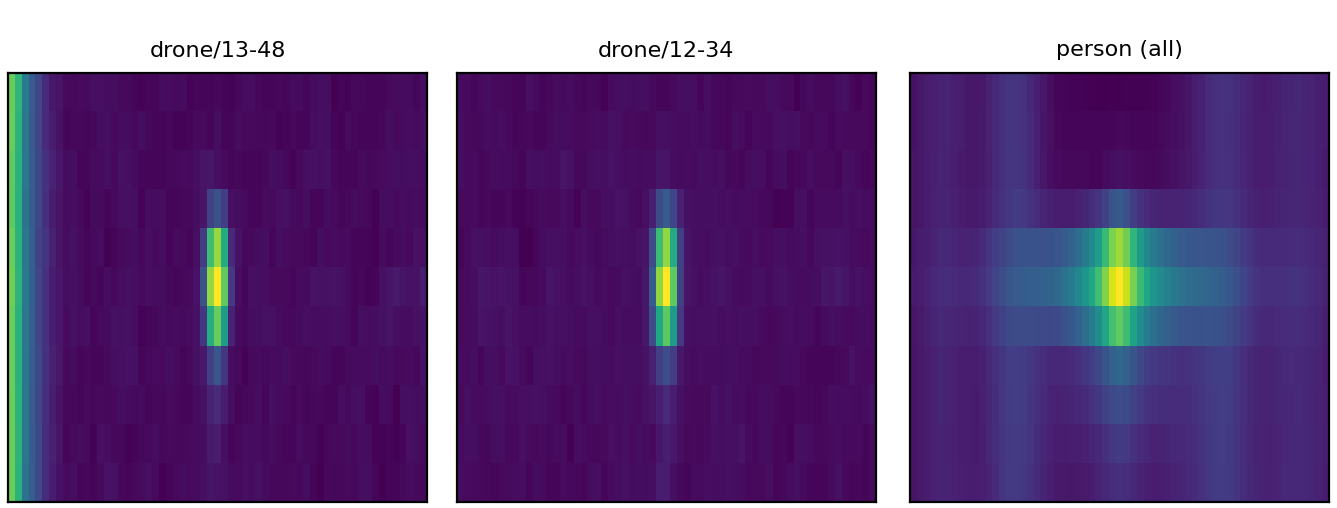
\includegraphics[width=\columnwidth]{session_13-48_compact.png}
\caption{Mean range-Doppler maps on one shared colour scale, each sample referenced to its own peak so the panels compare shape rather than level. \texttt{13-48} (left) carries a band of energy at the low edge of the Doppler window that a typical drone acquisition (centre) does not show, and the pedestrian mean (right) spreads along the same axis, where 79\% of held-out \texttt{13-48} samples are sent. The white curve is energy summed over range, the triangle the mean per-sample Doppler centroid, and the dashed line zero Doppler at bin 30.}
\label{fig:sessions}
\end{figure}

\begin{figure}[!tb]
\centering
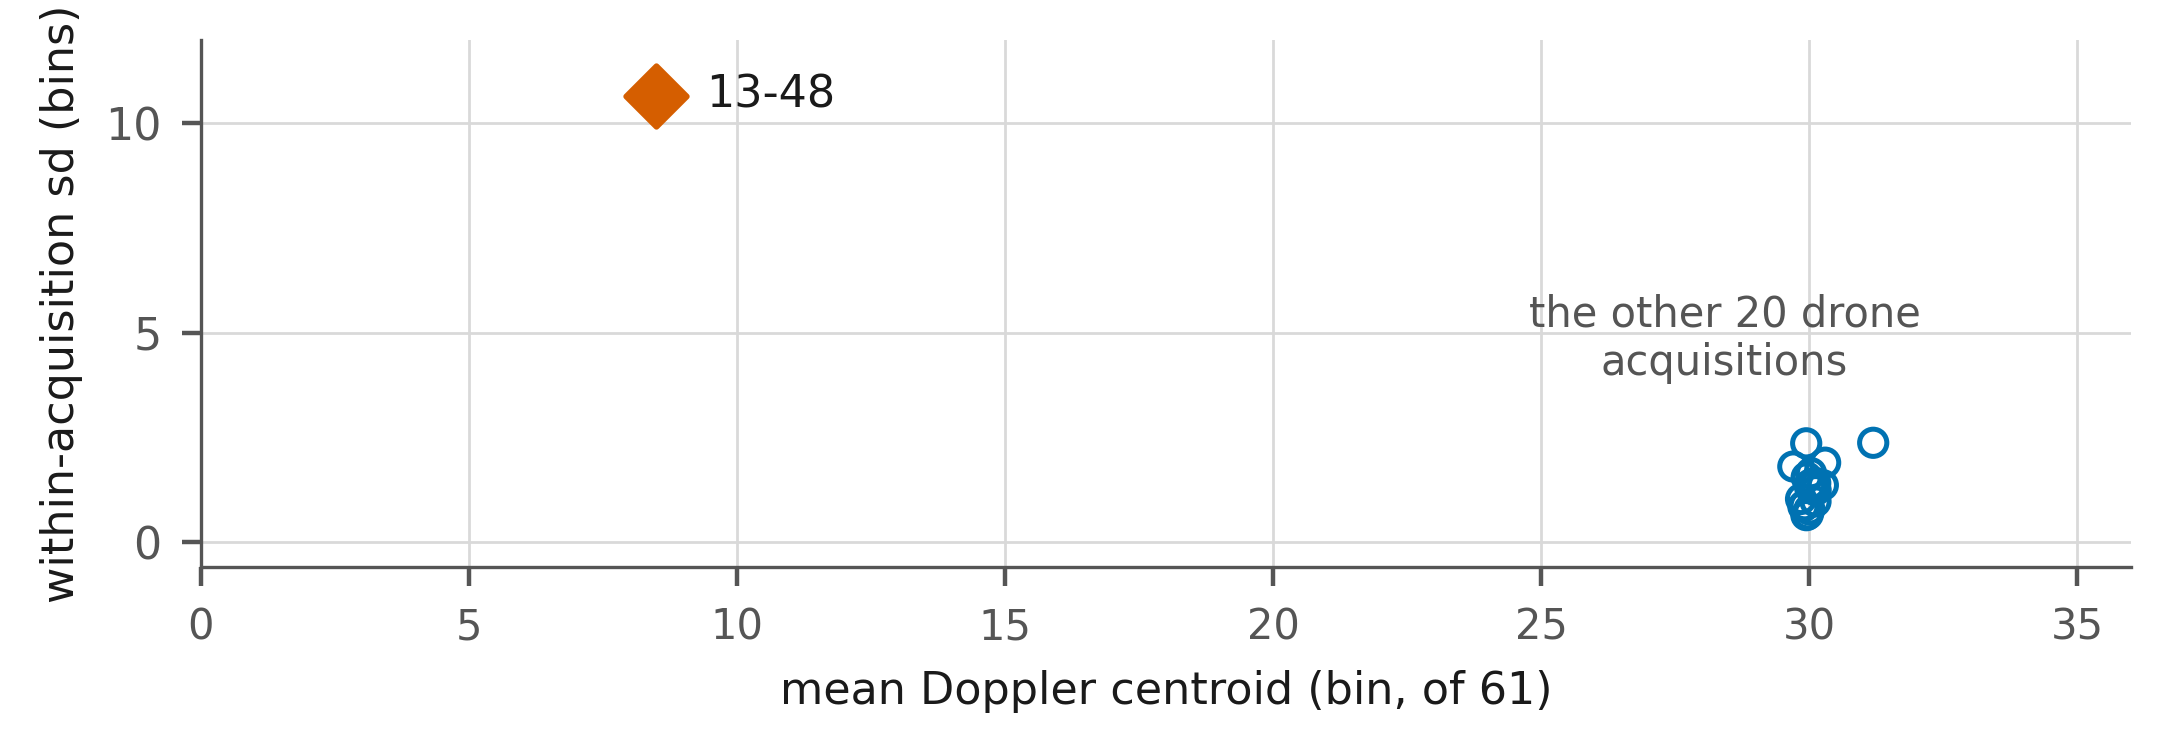
\includegraphics[width=\columnwidth]{doppler_by_acquisition.png}
\caption{Doppler centroid and within-acquisition spread of the 21 drone acquisitions. Twenty acquisitions cluster between bins 29.70 and 31.19 with spreads from 0.64 to 2.37 bins, whereas \texttt{13-48} lies at 8.50 with a spread of 10.64, separated on both axes.}
\label{fig:doppler}
\end{figure}

Twelve per-sample properties were compared through the standardized difference $d = (\bar{x}_{\mathrm{13\text{-}48}} - \bar{x}_{\mathrm{others}}) / s_{\mathrm{others}}$, the gap expressed in units of the spread among the other drone acquisitions. It is a descriptive effect size, not a test statistic. Five properties exceed $|d|=2$, and two of them dominate. The Doppler centroid lies at bin 8.50 against 30.04 ($d=-15.67$), and the peak Doppler bin at 7.58 against 30.01 ($d=-8.16$). Headroom, peak level, and dynamic range fall between $d=+2.07$ and $+2.57$, while range position, range spread, and energy extent differ little. The separation is therefore almost entirely a matter of Doppler position.

Fig.~\ref{fig:sessions} shows this difference in the mean samples, and Fig.~\ref{fig:doppler} shows it across all drone acquisitions. The within-acquisition Doppler spread of \texttt{13-48} is also more than four times that of any other drone acquisition. Measured against class centroids computed from the other acquisitions, all of its samples are still closest to the drone centroid. This agrees with the label but is not independent evidence for it.

The source publications describe three drone exercises, namely radial autopilot trajectories up to 3.1\,km, a circular trajectory at 800\,m, and a manually controlled free flight with variable speed and altitude~\cite{roldan2020,quevedo2019}. Manual free flight normally produces a wider spread of radial velocity than autopilot flight, and \texttt{13-48} is the only acquisition with markedly higher Doppler scatter, which makes it the most likely candidate. The publications give no timestamps, however, so a difference in how this recording was processed cannot be excluded.

\subsection{Coverage Test}
\label{sec:coverage}

\begin{table}[t]
\caption{Coverage Test Averaged Over Ten Seeds. Each Acquisition Is Excluded From Training, Then Half of It Is Reintroduced. Both Conditions Are Tested on the Same Reserved Half. The Two Controls Were Chosen After Inspecting Recall and Are Exploratory.}
\label{tab:coverage}
\centering
\setlength{\tabcolsep}{4pt}
\begin{ICICtable}
\begin{tabular}{@{}llccc@{}}
\toprule
Acquisition & Class & Held out & Half in training & Recovery \\
\midrule
\texttt{13-48} & drone      & 0.178 & \textbf{0.948} & \textbf{$+0.770$} \\
\texttt{11-23} & pedestrian & 0.800 & 0.856          & $+0.056$ \\
\texttt{15-37} & vehicle    & 0.837 & 0.845          & $+0.008$ \\
\bottomrule
\end{tabular}
\end{ICICtable}
\end{table}

To separate a lack of comparable training data from intrinsic difficulty, \texttt{13-48} is split in half. In the first condition the whole acquisition is excluded from training, and in the second one half is added to the training set. Both conditions are evaluated on the same reserved half ($N=197$). Over ten seeds, recall rises from 0.178 to 0.948, a recovery of 0.770 (Table~\ref{tab:coverage}). With the acquisition held out, 79\% of its samples are assigned to the pedestrian class, against 3\% when half of it is in training. Held-out recall ranges from 0.142 to 0.264 and half-in-training recall from 0.904 to 0.980, so the lowest value of the second condition exceeds the highest value of the first by 0.640. The two conditions are separated without any distributional assumption.

The failure therefore results from a lack of comparable training examples, not from an inherent inability to classify these samples. Because the added samples come from the same acquisition, the experiment cannot distinguish an out-of-distribution flight regime from an acquisition-specific signature or a per-recording processing difference. It does show that whatever this acquisition contains, and the other twenty lack, is both learnable and sufficient.

\subsection{Coverage Across All 52 Acquisitions}
\label{sec:controls}

\begin{figure}[!tb]
\centering
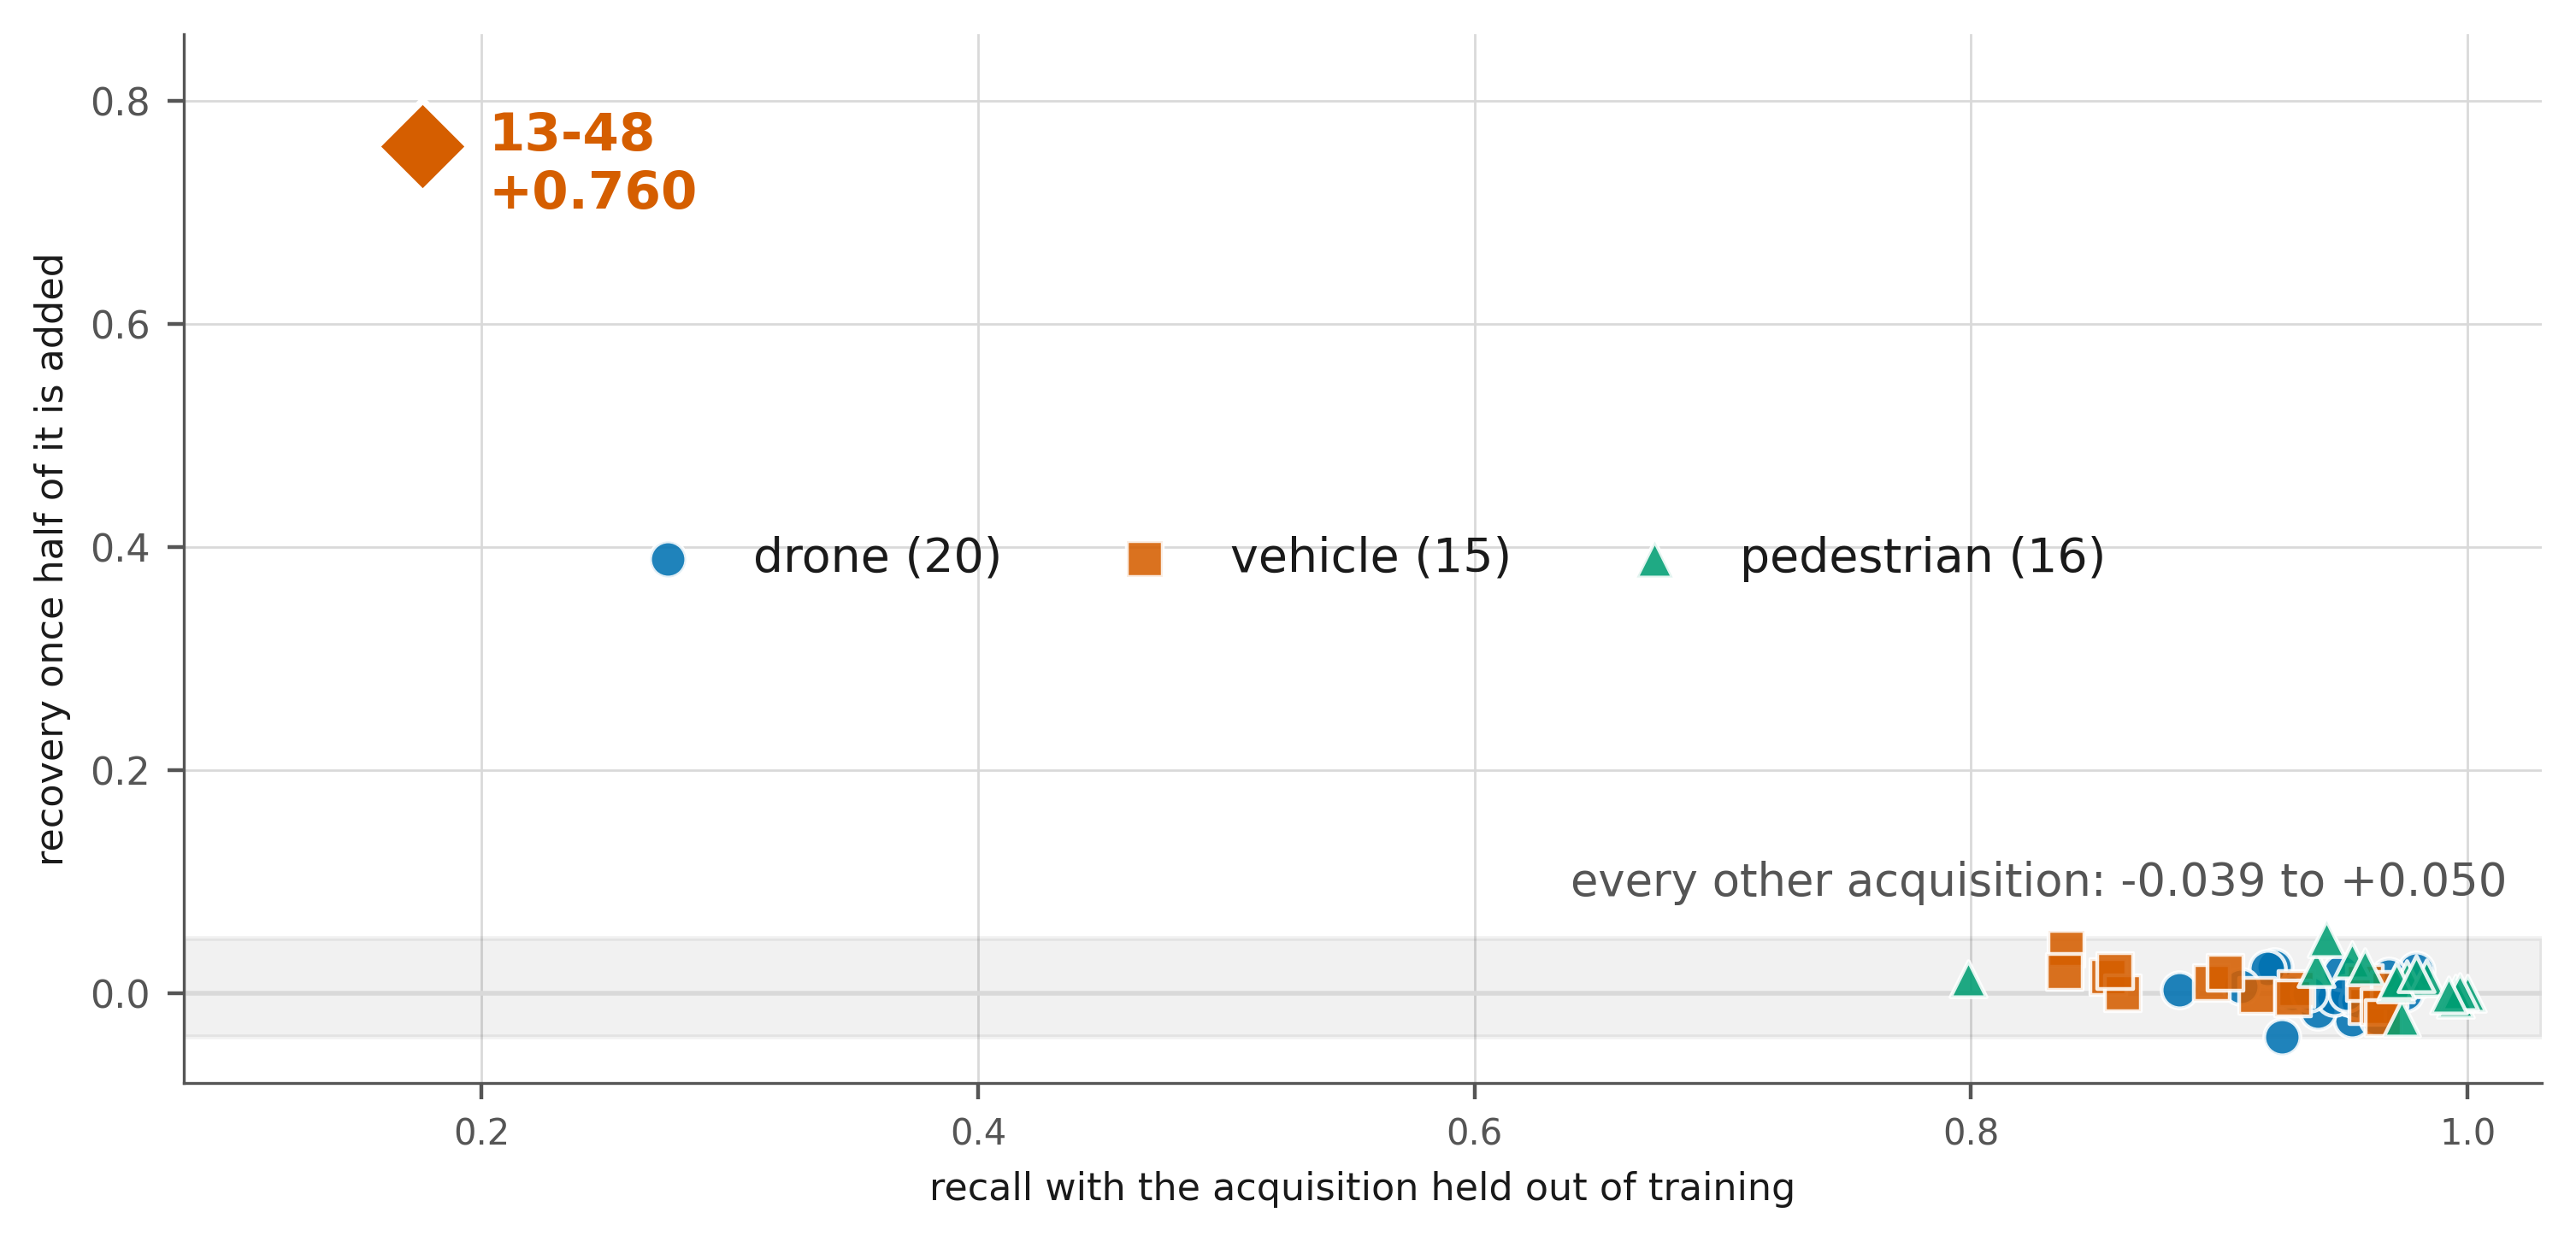
\includegraphics[width=\columnwidth]{recovery_by_acquisition.png}
\caption{Coverage test for all 52 acquisitions at three seeds, with recovery plotted against held-out recall. The shaded band spans the recoveries of the other 51 acquisitions, all of which have held-out recall of at least 0.79.}
\label{fig:recovery}
\end{figure}

A large recovery indicates a coverage failure only if such recoveries are rare. To avoid selection bias, the experiment was repeated for all 52 units at three seeds, 312 trainings in total (Fig.~\ref{fig:recovery}). The other 51 units recover between $-0.039$ and $+0.050$, with a standard deviation of 0.017. \textbf{None exceeds 0.050}, whereas \texttt{13-48} recovers 0.760, fifteen times the largest other value. Among the 20 other drone units the largest recovery is 0.024, and 16 of the 51 units show negative recovery, consistent with random variation around zero.

Regression to the mean offers an alternative explanation, since a unit that starts low has more room to improve. The horizontal axis of Fig.~\ref{fig:recovery} tests this. Across all 52 units, held-out recall and recovery correlate at $r=-0.927$, but this value is driven by \texttt{13-48}. For the other 51 units the correlation is $-0.282$ ($t=-2.06$, 49 degrees of freedom), which explains 8\% of the variance, and among the 23 units below 0.95 it is $-0.238$. A weak association exists, but it cannot account for a recovery of 0.760.

The weakest unit of each other class was also tested at ten seeds (Table~\ref{tab:coverage}). Pedestrian unit \texttt{11-23} ($N=154$) recovers 0.056 and vehicle unit \texttt{15-37} ($N=185$) recovers 0.008. Neither is unrepresented in training in the way \texttt{13-48} is. Unit \texttt{11-23} is an outlier in energy extent ($d=+3.4$) and 56.8\% of its frames lie nearest the \emph{drone} centroid, so it is confusable with another class rather than missing from training. No property separates \texttt{15-37} from the other vehicle acquisitions. An acquisition can thus be weak without being unrepresented, and the coverage test distinguishes the two cases.

In summary, the classifier fails on one acquisition because of an acquisition-specific coverage gap, not a class-wide weakness, and no other acquisition behaves this way.

\subsection{Approximate Temporal Context}
\label{sec:inputgap}

This subsection tests whether the failure is an artifact of single-frame input. It uses the compact network of Table~\ref{tab:arch}, not DopplerNet, and says nothing about how DopplerNet would perform on \texttt{13-48}. The compact network reaches 0.9335 with frame-level random five-fold cross-validation and 0.9537 on a single random partition, against 99.48\% reported for DopplerNet~\cite{roldan2020} and 98.08\% for the lighter reference~\cite{zhang2025}. These figures measure different quantities, and the gaps point in opposite directions.

DopplerNet's figure is a five-fold cross-validated mean over random subsets~\cite{roldan2020}, the same protocol as the 0.9335 above, which leaves a gap of 6.1 points that the protocol does not explain. Two differences remain. DopplerNet has 3,818,755 parameters against 101,139, and its input is an $11 \times 61 \times 3$ range-Doppler-time tensor that stacks three consecutive detections taken 400\,ms apart. The lighter reference differs in the other direction. Its 0.9808 is the peak validation accuracy of an 80/20 split without a separate test set~\cite{zhang2025}, that is, accuracy measured on the data used to choose the epoch. The 0.9537 reported here is test accuracy on data withheld from both training and model selection, using an architecture within 300 parameters of that reference on the same single-frame input. The two values are not comparable, and the more conservative definition is used here. Capacity and schedule do not explain the gap either. Across width multipliers of one, two, and three (up to 871,731 parameters) and budgets of 40 and 80 epochs, the best of the six configurations reaches 0.9546.

Users of the release cannot close the input gap. The archive provides one CFAR crop per detection without a timestamp or frame counter, and the only ordering is the trailing integer of each file name. A recent multiradar drone dataset likewise orders its files only through a file-name index~\cite{han2026}. The 400\,ms triplets therefore cannot be rebuilt from the public data, and a headline accuracy that relies on them cannot be reproduced.

\begin{table}[t]
\caption{Approximate Three-Frame Context Over Ten Seeds, With Random-Split Accuracy Over Three Seeds. $d$ Is the Mean Index Distance of Companion Frames From the Center Frame. All Arms Use the Compact Network, Not DopplerNet.}
\label{tab:temporal}
\centering
\setlength{\tabcolsep}{3pt}
\begin{ICICtable}
\begin{tabular}{@{}llccc@{}}
\toprule
Arm & Companions & $d$ & Random split & \texttt{13-48} recall \\
\midrule
single  & none            & n/a  & 0.9516 $\pm$ 0.0046 & 0.2379 $\pm$ 0.0428 \\
index   & adjacent        & 1.00 & 0.9794 $\pm$ 0.0016 & 0.3673 $\pm$ 0.0661 \\
clean   & same split tag  & 2.57 & 0.9731 $\pm$ 0.0080 & 0.4634 $\pm$ 0.0970 \\
shuffle$^{\dagger}$ & folder-wide & n/a & 0.9932 $\pm$ 0.0016 & 0.5435 $\pm$ 0.1257 \\
\bottomrule
\multicolumn{5}{@{}p{0.95\columnwidth}@{}}{\scriptsize $^{\dagger}$Companions may include other test frames. The arm is transductive, so its accuracy is not comparable with a deployed system.}
\end{tabular}
\end{ICICtable}
\end{table}

The formulation is therefore approximated. Triplets are formed within each folder from consecutive file-name integers and never across a gap, which yields 17,221 triplets from 17,485 frames, 391 of them in \texttt{13-48}. Four arms are compared at ten shared seeds on the same center frames, so the comparison is paired sample by sample (Table~\ref{tab:temporal}). The \emph{single} arm uses the center frame alone, \emph{index} adds its two index-adjacent neighbors, \emph{clean} adds the nearest neighbors that carry the center frame's own split tag so that no window crosses the partition, and \emph{shuffle} adds two random frames from the same folder. The multi-frame arms keep channels, folders, labels, and sample counts fixed, and the extra input channels raise the parameter count to 102,291.

Three-frame input raises random-split accuracy from 0.9516 to 0.9794, within 0.0014 of the 0.9808 reported for the lighter published model. The classifier still fails on \texttt{13-48}, whose held-out recall rises only from 0.238 to 0.367, a paired gain of $+0.129$ over ten seeds ($t=+4.82$). Most of its frames are still misclassified. \textbf{The failure is therefore not an artifact of single-frame input, and it persists while aggregate accuracy rises by 2.8 points.} Even the shuffle arm, at 0.9932 accuracy, leaves the acquisition at 0.544, far below the 0.948 reached once it is represented in training.

A sliding window over a frame-level random split also places test frames inside training inputs on a large scale. Of the training triplets, 50.6\% contain at least one test frame, and 82.7\% of test frames appear inside some training input under index order, against 68.4\% with shuffled companions. The \emph{clean} arm, which has no such overlap, measures the effect. Removing the overlap lowers accuracy by only 0.0063, from 0.9794 to 0.9731, which is within the spread of either arm, and three frames still outperform one by 0.0215. Although four fifths of the test set appears somewhere in training, the resulting inflation is well under one point.

Recall on \texttt{13-48} rises with the distance between companions and the center frame, from 0.367 for adjacent frames to 0.463 for same-tag frames at a mean distance of 2.57 and 0.544 for companions drawn from the whole folder. Adjacent detections are nearly redundant, whereas distant ones sample the large variability of this acquisition. The index and shuffle arms differ by 0.176 ($t=-4.35$ over ten paired seeds), so the trailing integer tracks acquisition order closely enough to matter. Because the shuffle arm draws on other test frames at inference, the comparison rests on the index arm. Even that arm is centered on the frame being classified, so a streaming system could form it only by delaying each decision by one frame, the latency noted for DopplerNet's own three-frame input~\cite{roldan2020}.

\subsection{Candidate Mechanisms}
\label{sec:discussion}

The coverage result does not identify which physical or processing factor makes such coverage necessary. The release provides only \emph{relative} Doppler within each crop, so absolute velocity cannot be measured, and the anomaly could stem from flight dynamics or from recording-specific processing. Only the former would affect deployment, and where deployment matches the benchmark distribution, frame-level evaluation may still be adequate.

A compression study in the released artifact found that fourfold Doppler aggregation raised held-out recall on \texttt{13-48} from 0.222 to 0.398 over ten seeds, with no gain on the standard split, and it helped only three of five individual acquisitions. As with class-level effects of compression in vision~\cite{hooker2019,tran2022}, the effect is uneven and becomes visible only below the aggregate level, so this aggregation is not recommended in general.

Four physically motivated mechanisms were also examined, and none was supported, so the physical cause is left unresolved. Rotor sideband loss cannot be assessed within the Doppler span of the crops. Low redundancy from compact energy was considered without a supporting effect. Dynamic-range headroom correlates with per-acquisition recall (Pearson $r=-0.62$), but the correlation falls to $-0.16$ without \texttt{13-48}, which has the largest headroom at 42.5\,dB against a class median near 26\,dB. Doppler position insensitivity is not repaired by shift augmentation of $\pm4$, $\pm8$, and $\pm16$ bins, which gives recalls of 0.1608, 0.1613, and 0.1603 against 0.2214 without augmentation.

\subsection{Limitations}

Both principal findings rest on the same acquisition, so the effective sample size at the level of flight regimes is one, from one dataset, one radar, and one drone platform, and \texttt{13-48} holds 7.8\% of the drone samples. The 52-unit sweep removes the reliance on hand-picked controls but says nothing about how common such acquisitions are elsewhere, and it uses three seeds rather than the ten of the focal experiment. Other architectures and other radars remain untested. Because neither a wider network nor three-frame input lifts this acquisition above 0.367, the failure would be expected to survive a change of architecture, but this has not been shown.

% =====================================================================
\section{Conclusion}

On the Real Doppler RAD-DAR benchmark, grouping frames by inferred acquisition reveals heterogeneity that aggregate frame-level accuracy misses. One drone acquisition out of twenty-one reaches 0.249 out-of-fold recall, while the other twenty reach 0.90 or more. Adding half of it to training raises recall on the other half from 0.178 to 0.948, a recovery that no other of the 52 acquisitions approaches, and the failure persists with three-frame input. The acquisition is distinguished by the Doppler position and spread of its energy. These results form a benchmark-specific case study rather than a general law. They nonetheless support reporting per-acquisition performance whenever a dataset is assembled from continuous recordings, since it costs only one cross-validation pass. Future work will apply the audit to other radar benchmarks and architectures. Code, partition files, per-stage reports, and a script that rechecks every number against its tolerance are released at \codeurl{}~\cite{artefact2026}.


\section*{ACKNOWLEDGMENT}

The authors thank C.~R.~del-Blanco, I.~Roldan and their colleagues at the Universidad Polit\'ecnica de Madrid for collecting the Real Doppler RAD-DAR database and for releasing it publicly. This study is an audit of that resource and would not have been possible without it.

% =====================================================================
\begin{thebibliography}{00}

\bibitem{ahmad2024} B.~I.~Ahmad, C.~Rogers, S.~Harman \emph{et al.}, ``A review of automatic classification of drones using radar: Key considerations, performance evaluation and prospects,'' \emph{IEEE Aerosp. Electron. Syst. Mag.}, vol.~39, no.~2, pp.~18--33, 2024.

\bibitem{liaquat2025imm} S.~Liaquat, F.~A.~Butt, F.~A.~Nasir \emph{et al.}, ``SDR-based metal classification using spectrogram images from micro-Doppler signatures,'' \emph{IEEE Instrum. Meas. Mag.}, vol.~28, no.~3, pp.~22--29, May 2025.

\bibitem{mustafa2026} S.~E.~Mustafa, S.~Liaquat, I.~H.~Abbasi, and A.~Hasan, ``Feature-level robustness analysis of physics-guided micro-Doppler descriptors for classification of drones and birds,'' \emph{J. Inf. Intell.}, 2026, in press, doi:10.1016/j.jiixd.2026.07.004.

\bibitem{roldan2020} I.~Roldan, C.~R.~del-Blanco, \'A.~Duque de Quevedo \emph{et al.}, ``DopplerNet: A convolutional neural network for recognising targets in real scenarios using a persistent range--Doppler radar,'' \emph{IET Radar Sonar Navig.}, vol.~14, no.~4, pp.~593--600, 2020.

\bibitem{zhang2025} L.~Zhang, G.~Tu, Y.~Xu, and X.~Zhou, ``A lightweight CNN-based method for micro-Doppler feature-based UAV detection and classification,'' \emph{Electronics}, vol.~14, no.~24, Art.~no.~4831, 2025.

\bibitem{kapoor2023} S.~Kapoor and A.~Narayanan, ``Leakage and the reproducibility crisis in machine-learning-based science,'' \emph{Patterns}, vol.~4, no.~9, Art.~no.~100804, 2023.

\bibitem{buchman2022} D.~Buchman, M.~Drozdov, T.~Krilavi\v{c}ius \emph{et al.}, ``Pedestrian and animal recognition using Doppler radar signature and deep learning,'' \emph{Sensors}, vol.~22, no.~9, Art.~no.~3456, 2022.

\bibitem{quevedo2019} \'A.~Duque de Quevedo, F.~Ib\'a\~nez Urzaiz, J.~Gismero Menoyo \emph{et al.}, ``Drone detection and radar-cross-section measurements by RAD-DAR,'' \emph{IET Radar Sonar Navig.}, vol.~13, no.~9, pp.~1437--1447, 2019.

\bibitem{kim2016} Y.~Kim and T.~Moon, ``Human detection and activity classification based on micro-Doppler signatures using deep convolutional neural networks,'' \emph{IEEE Geosci. Remote Sens. Lett.}, vol.~13, no.~1, pp.~8--12, 2016.



\bibitem{liaquat2024tut} S.~Liaquat, N.~M.~Mahyuddin, and I.~H.~Naqvi, ``An end-to-end modular framework for radar signal processing: A simulation-based tutorial,'' \emph{IEEE Aerosp. Electron. Syst. Mag.}, vol.~39, no.~9, pp.~98--118, Sep. 2024.

\bibitem{varga2024a} D.~Varga, ``Critical analysis of data leakage in WiFi CSI-based human action recognition using CNNs,'' \emph{Sensors}, vol.~24, no.~10, Art.~no.~3159, 2024.

\bibitem{varga2024b} D.~Varga, ``Mitigating data leakage in a WiFi CSI benchmark for human action recognition,'' \emph{Sensors}, vol.~24, no.~24, Art.~no.~8201, 2024.

\bibitem{chen2025} L.~Chen, N.~Zhu, H.~Chen \emph{et al.}, ``A causality-inspired single-source domain generalized method for low-slow-small threat target recognition through holographic Doppler radar,'' \emph{Expert Syst. Appl.}, vol.~287, Art.~no.~128104, 2025.

\bibitem{bai2026} B.~Bai, L.~Xue, M.~Xue \emph{et al.}, ``Open-set recognition of radar one-dimensional range profiles based on attention mechanism and multi-task joint training,'' \emph{IET Radar Sonar Navig.}, vol.~20, no.~1, Art.~no.~e70121, 2026.

\bibitem{dietterich1998} T.~G.~Dietterich, ``Approximate statistical tests for comparing supervised classification learning algorithms,'' \emph{Neural Comput.}, vol.~10, no.~7, pp.~1895--1923, 1998.

\bibitem{nadeau2003} C.~Nadeau and Y.~Bengio, ``Inference for the generalization error,'' \emph{Mach. Learn.}, vol.~52, no.~3, pp.~239--281, 2003.

\bibitem{hooker2019} S.~Hooker, A.~Courville, G.~Clark \emph{et al.}, ``What do compressed deep neural networks forget?'' 2019, \emph{arXiv:1911.05248}.

\bibitem{tran2022} C.~Tran, F.~Fioretto, J.-E.~Kim, and R.~Naidu, ``Pruning has a disparate impact on model accuracy,'' in \emph{Proc. Adv. Neural Inf. Process. Syst. (NeurIPS)}, vol.~35, 2022, pp.~17652--17664.

\bibitem{han2026} S.-K.~Han and Y.-H.~Jung, ``A time-synchronized multi-sensor drone dataset acquired from multiple radars and RF receiver,'' \emph{Sci. Data}, vol.~13, Art.~no.~407, 2026.

\ifblind
\bibitem{artefact2026} Author(s) withheld for blind review, ``Code and analysis for this paper,'' archived artefact, 2026.
\else
\bibitem{artefact2026} G.~Mustafa, ``Code and analysis for \emph{Acquisition-level evaluation of deep learning for range-Doppler radar target recognition},'' Zenodo, 2026, doi:10.5281/zenodo.23118075. [Online]. Available: \url{https://github.com/falcon-colab/rdrd-acquisition-coverage}
\fi

\end{thebibliography}

\end{document}
